\section{EKG-Verstärkerschaltung} % (fold)
\label{sec:EKG-Verstärkerschaltung}
\begin{frame}
\frametitle{EKG-Verstärkerschaltung}
\framesubtitle{}
    \begin{block}{Versuch}
        \begin{itemize}
            \item Verbinden aller Einzelbauteile
            \item Aufnahme eines EKGs
            \item Bodediagramm der Gesamtschaltung
        \end{itemize}        
    \end{block}
    \begin{figure}[H]
    \begin{center}
            \includegraphics[scale=0.1]{./img/schaltung/gesamt.png}
    \end{center}
    \end{figure}
\end{frame}
\begin{frame}
\frametitle{Enstehung der Potentialdifferenz}
\framesubtitle{}
    \begin{block}{Erzeugung}
         \begin{itemize}
             \item Sinusknoten regt durch elektrische Signale verschiedene
             Teile der Herzmuskeln an
         \end{itemize}
    \end{block}
    \begin{block}{Wie entsteht die Differenz?}
        \begin{itemize}
            \item Signale brauchen verschieden lang um zu verschiedenen Teilen
            des Körpers zu kommen $\rightarrow$ Potentialdifferenz
        \end{itemize}
    \end{block}
\end{frame}
\begin{frame}
\frametitle{Bilder}
\framesubtitle{}
    \begin{figure}[H]
    \begin{center}
            \includegraphics[]{./img/oszi/scope_13.png}
    \end{center}
    \end{figure}
    
\end{frame}
\framesubtitle{}
    \begin{figure}[H]
    \begin{center}
            \includegraphics[]{./img/oszi/scope_14.png}
    \end{center}
    \end{figure}
    
\end{frame}
\framesubtitle{}
    \begin{figure}[H]
    \begin{center}
            \includegraphics[]{./img/schaltung/wellen.png}
    \end{center}
    \end{figure}
    \begin{block}{}
         \begin{itemize}
             \item $PQ$-Strecke:
             \item $ST$-Strecke:
         \end{itemize}
    \end{block}
\end{frame}
\begin{frame}
\frametitle{Verfolgung des Signals}
\framesubtitle{}
\begin{columns}[c]
\column{0.4\textwidth}
\begin{block}{Signalmodulation:}
     \begin{itemize}
         \item Gelb: Eingangssignal\\
         nach Differenzverstärker
         \item Grün: Verstärktes Signal\\
         nach Invertierendem Verstärker
         \item Lila: Gefilltertes Signal\\
         nach Tiefpassfilter
     \end{itemize}
\end{block}
\column{0.6\textwidth}
\begin{figure}[H]
\begin{center}
        \includegraphics[scale=0.15]{./img/oszi/scope_22.png}
\end{center}
\end{figure}
\end{columns}
\end{frame}
\begin{frame}
\frametitle{Bode-Diagramm}
\framesubtitle{}
    \begin{figure}[H]
    \begin{center}
            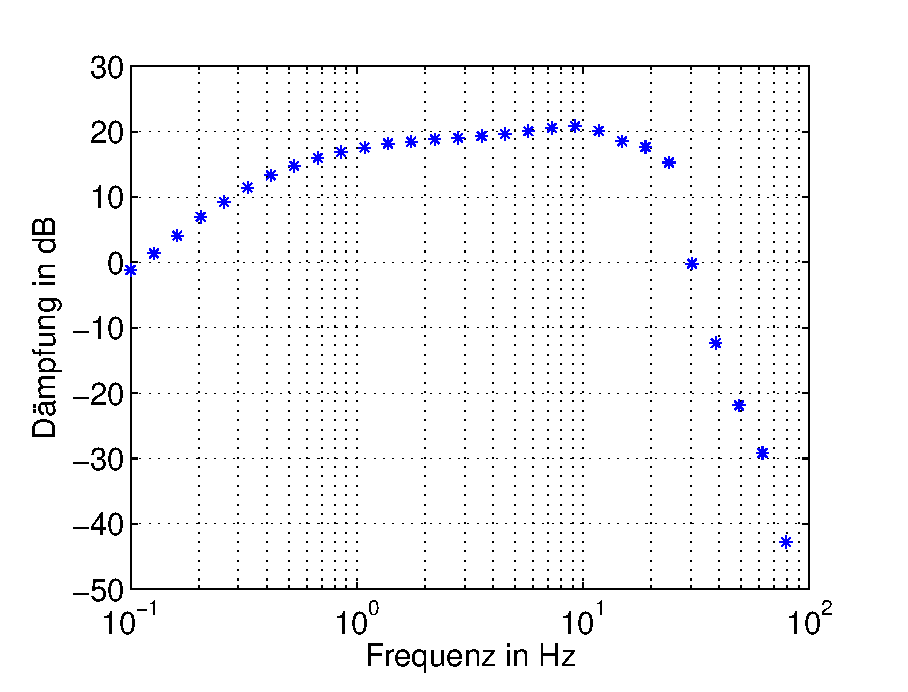
\includegraphics[scale=0.2]{./img/plots/Auf_5_bode_db.eps}
    \end{center}
    \end{figure}
\end{frame}

% section EKG-Verstärkerschaltung (end)
